\documentclass[a4paper,twoside,openright,titlepage]{article}

%-------------------------------------------------------
% Paquetes incluidos
%-------------------------------------------------------
%\usepackage[spanish]{babel} 	% Para el idioma.
\usepackage[utf8]{inputenc}		% Para escribir con acentos
\usepackage{graphicx} 			% Imagenes
\usepackage{colortbl} 			% Color en tablas
\usepackage{anysize} 			% Margenes
%\usepackage{amsmath} 			% Simbolos matematicos
\usepackage{fancyhdr} 			% Cabecera y pie de pagina
\usepackage{emptypage}
\usepackage{pdfpages}			% Para agregar pdf's externos
\usepackage{float} 				% Para colocar las imagenes forzando.
\usepackage{multirow, array} 	% Para las tablas
\usepackage{listings}			% Para el codigo fuente
\usepackage{caption}				% Personalizar los caption
\usepackage[bookmarks]{hyperref} %hypervinculos del indice
\usepackage[nohyperlinks,smaller,withpage]{acronym}
%--------------------------------------------------------
% Editor de hipervinculo
%--------------------------------------------------------
\hypersetup{
    colorlinks,
    citecolor=black,
    filecolor=black,
    linkcolor=black,
    urlcolor=black
}
%----
%--------------------------------------------------------
% listas con mayor profundidad
%--------------------------------------------------------
\usepackage{enumitem}
\newlist{longenum}{enumerate}{6}
\setlist[longenum,1]{label=\arabic*.}
\setlist[longenum,2]{label=\textit{\alph*})}
\setlist[longenum,3]{label=\arabic*)}
\setlist[longenum,4]{label=\roman*.}
\setlist[longenum,5]{label=(\Alph*)}
\setlist[longenum,6]{label=\arabic*)}
% -------------------------------------------------------
% cabecera
%--------------------------------------------------------
\pagestyle{fancy} % seleccionamos un estilo cabecera
\fancyhead[RO,LE]{Arquitectura de Computadoras - Pipeline}
\fancyfoot[RO,LE] {\thepage}
\renewcommand{\headrulewidth}{0.1pt}	% El ancho de las lineas de separacion arriba
\renewcommand{\footrulewidth}{0.1pt}
% -------------------------------------------------------
% Establezco los margenes
%--------------------------------------------------------
\marginsize{2.5cm}{3cm}{2.5cm}{3cm}
%--------------------------------------------------------
% Para hacer el 4to nivel de subtitulo
%--------------------------------------------------------
\usepackage{titlesec}
\setcounter{secnumdepth}{4}
\titleformat{\paragraph}
{\normalfont\normalsize\bfseries}{\theparagraph}{1em}{}
\titlespacing*{\paragraph}
{0pt}{3.25ex plus 1ex minus .2ex}{1.5ex plus .2ex}
%--------------------------------------------------------
% Personalizacion del codigo fuente
%--------------------------------------------------------
%\lstset{ %
% backgroundcolor=\color{white},  Elige el color de fondo; Se debe agregar \usepackage{color} or \usepackage{xcolor}
%  basicstyle=\footnotesize,        % El tamaño de la fuente usada para el codigo
%  breakatwhitespace=false,         % sets if automatic breaks should only happen at whitespace
%  breaklines=true,                 % sets automatic line breaking
%  captionpos=b,                    % sets the caption-position to bottom
%  commentstyle=\color{mygreen},    % comment style
%  deletekeywords={...},            % if you want to delete keywords from the given language
%  escapeinside={\%*}{*)},          % if you want to add LaTeX within your code
%  extendedchars=true,              % lets you use non-ASCII characters; for 8-bits encodings only, does not work with UTF-8
%  frame=single,                    % adds a frame around the code
%  keepspaces=true,                 % keeps spaces in text, useful for keeping indentation of code (possibly needs columns=flexible)
%  keywordstyle=\color{blue},       % keyword style
%  language=Octave,                 % the language of the code
%  morekeywords={*,...},            % if you want to add more keywords to the set
%  numbers=left,                    % where to put the line-numbers; possible values are (none, left, right)
%  numbersep=5pt,                   % how far the line-numbers are from the code
%  numberstyle=\tiny\color{mygray}, % the style that is used for the line-numbers
%  rulecolor=\color{black},         % if not set, the frame-color may be changed on line-breaks within not-black text (e.g. comments (green here))
%  showspaces=false,                % show spaces everywhere adding particular underscores; it overrides 'showstringspaces'
%  showstringspaces=false,          % underline spaces within strings only
%  showtabs=false,                  % show tabs within strings adding particular underscores
%  stepnumber=2,                    % the step between two line-numbers. If it's 1, each line will be numbered
%  stringstyle=\color{mymauve},     % string literal style
%  tabsize=2,                       % sets default tabsize to 2 spaces
%  title=\lstname                   % show the filename of files included with \lstinputlisting; also try caption instead of title
\usepackage{color}
\definecolor{gray97}{gray}{.97}
\definecolor{gray75}{gray}{.75}
\definecolor{gray45}{gray}{.45}
\definecolor{gray25}{gray}{.25}
%------------------------------------------------------
% Para codigo JAVA
%------------------------------------------------------
\lstset{ 
language=Java,
frame=single,
framerule=0pt,
aboveskip=0.5cm,
framextopmargin=3pt,
framexbottommargin=3pt,
framexleftmargin=0.4cm,
framesep=0pt,
rulesep=.4pt,
backgroundcolor=\color{gray97},
rulesepcolor=\color{black},
%
stringstyle=\ttfamily,
showstringspaces = false,
basicstyle=\small\ttfamily,
commentstyle=\color{gray45},
keywordstyle=\bfseries,
%
numbers=left,
numbersep=15pt,
numberstyle=\tiny,
numberfirstline = false,
breaklines=true
}
%--------------------------------------------------------
% Para codigo de C
%--------------------------------------------------------
\lstdefinestyle{customC}{
  belowcaptionskip=1\baselineskip,
  breaklines=true,
  frame=L,
  xleftmargin=\parindent,
  language=C,
  showstringspaces=false,
  basicstyle=\footnotesize\ttfamily,
  keywordstyle=\bfseries\color{green!40!black},
  commentstyle=\itshape\color{purple!40!black},
  identifierstyle=\color{blue},
  stringstyle=\color{orange},
   captionpos=b,
}
%--------------------------------------------------------
% Para consola
%--------------------------------------------------------
\lstdefinestyle{consola}
{basicstyle=\scriptsize\bf\ttfamily,
numbers=none,
}
%--------------------------------------------------------
% Para codigo en asm
%--------------------------------------------------------
\lstdefinestyle{customasm}{
  belowcaptionskip=1\baselineskip,
  frame=L,
  xleftmargin=\parindent,
  language=[x86masm]Assembler,
  basicstyle=\footnotesize\ttfamily,
  commentstyle=\itshape\color{purple!40!black},
}
%--------------------------------------------------------
% Personalizo el caption del listings
%--------------------------------------------------------
%\DeclareCaptionFont{white}{ \color{white} }
%\DeclareCaptionFormat{listing}{
%  \colorbox[cmyk]{0.43, 0.35, 0.35,0.01 }{
%    \parbox{\textwidth}{\hspace{15pt}#1#2#3}
%  }
%}
%\captionsetup[lstlisting]{ format=listing, labelfont=white, textfont=white, singlelinecheck=false, margin=0pt, font={bf,footnotesize} }
%--------------------------------------------------------
% Comienzo del documento
%--------------------------------------------------------
\begin{document}
	
	\renewcommand{\lstlistingname}{Código} %Listing x Codigo
	\thispagestyle{empty}
{\Huge \noindent Trabajo final\\ Arquitectura de computadoras}

\vspace{1cm}

{\Large \noindent Desarrollo de un pipeline de 5 etapas}
                  
\vspace{5cm}
\hrule                  
\vspace{0.2cm}
{\noindent Desarrollo de un pipeline de 5 etapas\bigskip
\\Unidades de detecci\'on de riesgo\bigskip
\\Unidad de debug a trav\'es de UART\bigskip
\\Validaci\'on y verificaci\'on de funcionamiento}
\vspace{0.2cm}
\hrule 


\vfill
\Large
\begin{center}
  \begin{tabular}{| p{5cm} | p{7cm} |}
    \hline
    Cantidad de Páginas    & \pageref{LastPage}  \\
    Fecha                  & Abril de 2014\\
    Lugar                  & Córdoba, Argentina\\  
    \hline    
    \end{tabular}
\end{center}

\bigskip
	Autores\\
    \textit{Alfonzo, Marcos}\\
    \textit{Cueva, Martin}\\	
    \textit{Morales, Nicolas}

\newpage


	\tableofcontents 	% Agrega el indice
%--------------------------------------------------------
% Contenido
%--------------------------------------------------------
	
	\newpage
\section{Introducc\'ion}

Utilizando verilog, se realiza un proyecto para la entrega del trabajo final de la materia arquitectura de computadoras 2012. El proyecto consiste en la construcci\'on de un pipeline de 5 etapas, capaz de decodificar un c\'odigo previamente cargado y que este sea capaz de procesarlo llegando hasta la ejecución. Por último, con fines de evaluaci\'on y verficaci\'on, embeber el c\'odigo desarrollado en una fpga y correr un programa desarrollado que demuestre el funcionamiento.

\subsection{IDE}
El entorno de desarrollo utilizado para el desarrollo del c\'odigo del pipeline es el \texttt{Project Navigator, release version 14.4 (lin), Aplication version:P49d}.
Para desarrolar la interfaz gr\'afica de debug se utiliz\'o el editor de interfaces \texttt{glade} y se program\'o la recepci\'on de datos en \texttt{python 2.7}. 

\subsection{SVN}
Se llev\'o a cabo el desarrallo del software utilizando un servidor svn para el control de cambios, que facilit\'o la tarea a la hora de volver hacia ``c\'odigo estable'' y desde all\'i retomar el desarrollo.

\subsection{Placa de desarrollo}
Para embeber el c\'odigo se utiliz\'o la placa de desarrollo de \texttt{Digilent, Nexys™3 Spartan-6 FPGA Board} con frecuencia de 100 MHZ. Las caracter\'isticas de la placa se detallan en la figura \ref{fig:digilent}.
\begin{figure}[H]
\centering
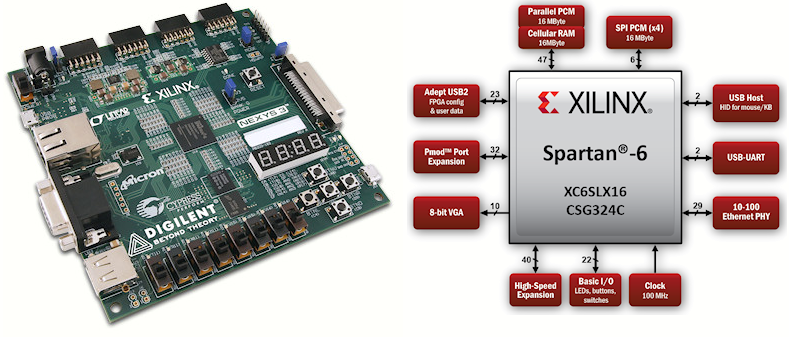
\includegraphics[scale=0.5]{img/digilent}
\caption{Placa de desarrollo}
\label{fig:digilent}
\end{figure} 		 
\newpage		

\subsection{Set de instrucciones implementado}

Para comenzar con el trabajo pr\'actico necesitamos saber cuales son las instrucciones que entran en juego en el pipeline. Una vez hecho esto podemos comenzar primero por un parser que verifique el estado de las instrucciones (si están correctamente escritas), para luego ejecutarlas con el pipeline.

\subsubsection{Instrucciones}
\textbf{Tipo I}\\

\texttt{LW (Load word)}

\begin{lstlisting}[style=consola]
32                             16                               0
+-+-+-+-+-+-+-+-+-+-+-+-+-+-+-+-+-+-+-+-+-+-+-+-+-+-+-+-+-+-+-+-+
|1 0 0 0 1 1|   base  |   rt    |              offset           |
+-+-+-+-+-+-+-+-+-+-+-+-+-+-+-+-+-+-+-+-+-+-+-+-+-+-+-+-+-+-+-+-+
+----6------+----5----+---5-----+---------------16--------------+

Formato: LW rt,offset(base)
Proposito: Guarda una palabra desde memoria a registro.
Descripcion: rt <- memory[base+offset]
\end{lstlisting}

\texttt{SW(store word)}

\begin{lstlisting}[style=consola]
32                             16                               0
+-+-+-+-+-+-+-+-+-+-+-+-+-+-+-+-+-+-+-+-+-+-+-+-+-+-+-+-+-+-+-+-+
|1 0 1 0 1 1|  base   |   rt    |             offset            |
+-+-+-+-+-+-+-+-+-+-+-+-+-+-+-+-+-+-+-+-+-+-+-+-+-+-+-+-+-+-+-+-+
+----6------+---5-----+---5-----+---------------16--------------+

Formato: SW rt,offset(base)
Proposito: Guarda palabra en memoria.
Descripcion: memory[base+offset] <- rt
\end{lstlisting}

\texttt{ADDI (Add Inmediate Word)}

\begin{lstlisting}[style=consola]
32                             16                               0
+-+-+-+-+-+-+-+-+-+-+-+-+-+-+-+-+-+-+-+-+-+-+-+-+-+-+-+-+-+-+-+-+
|0 0 1 0 0 0|   rs    |   rt    |            inmediate          |
+-+-+-+-+-+-+-+-+-+-+-+-+-+-+-+-+-+-+-+-+-+-+-+-+-+-+-+-+-+-+-+-+
+----6------+---5-----+---5-----+---------------16--------------+

Formato: ADDI rt, rs, inmediate
Proposito: Suma una constante a un entero de 32 bits. Si ocurre un overflow, then trap.
Descripcion: rt <- rs + inmediate
\end{lstlisting}

\texttt{ANDI (And Inmediate)}

\begin{lstlisting}[style=consola]
32                             16                               0
+-+-+-+-+-+-+-+-+-+-+-+-+-+-+-+-+-+-+-+-+-+-+-+-+-+-+-+-+-+-+-+-+
|0 0 1 1 0 0|   rs    |   rt    |            inmediate          |
+-+-+-+-+-+-+-+-+-+-+-+-+-+-+-+-+-+-+-+-+-+-+-+-+-+-+-+-+-+-+-+-+
+----6------+---5-----+---5-----+---------------16--------------+

Formato: ANDI rt, rs, inmediate
Proposito: Hace bit a bit la operacion logica AND con una constante.
Descripcion: rt <- rs AND immediate
\end{lstlisting}

\texttt{ORI (OR Inmediate)}

\begin{lstlisting}[style=consola]
32                             16                               0
+-+-+-+-+-+-+-+-+-+-+-+-+-+-+-+-+-+-+-+-+-+-+-+-+-+-+-+-+-+-+-+-+
|0 0 1 1 0 1|   rs    |   rt    |            inmediate          |
+-+-+-+-+-+-+-+-+-+-+-+-+-+-+-+-+-+-+-+-+-+-+-+-+-+-+-+-+-+-+-+-+
+----6------+---5-----+---5-----+---------------16--------------+

Formato: ORI rt, rs, immediate
Proposito: Hace una operacion logica OR bit a bit con una constante.
Descripcion: rd <- rs OR immediate
\end{lstlisting}

\texttt{XORI (Exclusive OR Immediate)}

\begin{lstlisting}[style=consola]
32                             16                               0
+-+-+-+-+-+-+-+-+-+-+-+-+-+-+-+-+-+-+-+-+-+-+-+-+-+-+-+-+-+-+-+-+
|0 0 1 1 1 0|   rs    |   rt    |            inmediate          |
+-+-+-+-+-+-+-+-+-+-+-+-+-+-+-+-+-+-+-+-+-+-+-+-+-+-+-+-+-+-+-+-+
+----6------+---5-----+---5-----+---------------16--------------+

Formato: XORI rt, rs, immediate
Proposito: Hace una operacion logica OR bit a bit con una constante.
Descripcion: rt <- rs XOR inmediate
\end{lstlisting}

\texttt{SLTI(Set on Less Than Inmediate)}

\begin{lstlisting}[style=consola]
32                             16                               0
+-+-+-+-+-+-+-+-+-+-+-+-+-+-+-+-+-+-+-+-+-+-+-+-+-+-+-+-+-+-+-+-+
|0 0 1 0 1 0|   rs    |   rt    |           inmediate           |
+-+-+-+-+-+-+-+-+-+-+-+-+-+-+-+-+-+-+-+-+-+-+-+-+-+-+-+-+-+-+-+-+
+----6------+---5-----+---5-----+---------------16--------------+

Formato: SLTI rt, rs, inmediate
Proposito: Guarda el resultado de la comparacion con la constante. Coloca 1 en rt si rs es menor que el inmediato.
Descripcion: rt <- (rs < inmediate)
\end{lstlisting}

\texttt{BEQ(Branch on Equal)}

\begin{lstlisting}[style=consola]
32                             16                               0
+-+-+-+-+-+-+-+-+-+-+-+-+-+-+-+-+-+-+-+-+-+-+-+-+-+-+-+-+-+-+-+-+
|0 0 0 1 0 0|   rs    |   rt    |             offset            |
+-+-+-+-+-+-+-+-+-+-+-+-+-+-+-+-+-+-+-+-+-+-+-+-+-+-+-+-+-+-+-+-+
+----6------+---5-----+---5-----+---------------16--------------+

Formato: BEQ rs, rt, offset
Proposito: Compara si son iguales y salta.
Descripcion: if (rs = rt) luego salta.
\end{lstlisting}

\texttt{BNE(Branch on Not Equal)}

\begin{lstlisting}[style=consola]
32                             16                               0
+-+-+-+-+-+-+-+-+-+-+-+-+-+-+-+-+-+-+-+-+-+-+-+-+-+-+-+-+-+-+-+-+
|0 0 0 1 0 1|   rs    |   rt    |          offset               |
+-+-+-+-+-+-+-+-+-+-+-+-+-+-+-+-+-+-+-+-+-+-+-+-+-+-+-+-+-+-+-+-+
+----6------+---5-----+---5-----+---------------16--------------+

Formato: BNE rs, rt, offset
Proposito: Compara si son distintos y salta.
Descripcion: if (rs != rt) luego salta.
\end{lstlisting}

\texttt{J(Jump)}

\begin{lstlisting}[style=consola]
32                             16                               0
+-+-+-+-+-+-+-+-+-+-+-+-+-+-+-+-+-+-+-+-+-+-+-+-+-+-+-+-+-+-+-+-+
|0 0 0 0 1 0|            instr_index                            |
+-+-+-+-+-+-+-+-+-+-+-+-+-+-+-+-+-+-+-+-+-+-+-+-+-+-+-+-+-+-+-+-+
+----6------+-----------------------26--------------------------+

Formato: J target
Proposito: Salto dentro de los siguientes 256 MB.
\end{lstlisting}

\texttt{ADD(Add Word)}

\begin{lstlisting}[style=consola]
32                             16                               0
+-+-+-+-+-+-+-+-+-+-+-+-+-+-+-+-+-+-+-+-+-+-+-+-+-+-+-+-+-+-+-+-+
|0 0 0 0 0 0|  rs     |  rt     |  rd     |0 0 0 0 0|1 0 0 0 0 0|
+-+-+-+-+-+-+-+-+-+-+-+-+-+-+-+-+-+-+-+-+-+-+-+-+-+-+-+-+-+-+-+-+
+----6------+----5----+----5----+---5-----+----5----+-----6-----+

Formato: ADD rd, rs, rt
Proposito: To add 32-bit integers. If overflow occurs, then trap.
Descripcion: rd <- rs + rt
\end{lstlisting}

\texttt{SUB(Subtract Word)}

\begin{lstlisting}[style=consola]
32                             16                               0
+-+-+-+-+-+-+-+-+-+-+-+-+-+-+-+-+-+-+-+-+-+-+-+-+-+-+-+-+-+-+-+-+
|0 0 0 0 0 0|   rs    |   rt    |   rd    |0 0 0 0 0|1 0 0 0 1 0|
+-+-+-+-+-+-+-+-+-+-+-+-+-+-+-+-+-+-+-+-+-+-+-+-+-+-+-+-+-+-+-+-+
+----6------+----5----+----5----+---5-----+----5----+-----6-----+

Formato: SUB rd, rs, rt
Proposito: Para restar enteros de 32 bits.
Descripcion: rd <- rs - rt
\end{lstlisting}

\texttt{AND (And)}

\begin{lstlisting}[style=consola]
32                             16                               0
+-+-+-+-+-+-+-+-+-+-+-+-+-+-+-+-+-+-+-+-+-+-+-+-+-+-+-+-+-+-+-+-+
|0 0 0 0 0 0|   rs    |   rt    |   rd    |0 0 0 0 0|1 0 0 1 0 0|
+-+-+-+-+-+-+-+-+-+-+-+-+-+-+-+-+-+-+-+-+-+-+-+-+-+-+-+-+-+-+-+-+
+----6------+----5----+----5----+---5-----+----5----+-----6-----+

Formato: AND rd, rs, rt
Proposito: Operacion logica AND bit a bit.
Descripcion: rd <- rs AND rt
\end{lstlisting}

\texttt{OR(or)}

\begin{lstlisting}[style=consola]
32                             16                               0
+-+-+-+-+-+-+-+-+-+-+-+-+-+-+-+-+-+-+-+-+-+-+-+-+-+-+-+-+-+-+-+-+
|0 0 0 0 0 0|   rs    |   rt    |   rd    |0 0 0 0 0|1 0 0 1 0 1|
+-+-+-+-+-+-+-+-+-+-+-+-+-+-+-+-+-+-+-+-+-+-+-+-+-+-+-+-+-+-+-+-+
+----6------+----5----+----5----+---5-----+----5----+-----6-----+

Formato: OR rd, rs, rt
Proposito: Operacion logica OR bit a bit.
Descripcion: rd <- rs OR rt
\end{lstlisting}

\texttt{XOR(Exclusive OR)}

\begin{lstlisting}[style=consola]
32                             16                               0
+-+-+-+-+-+-+-+-+-+-+-+-+-+-+-+-+-+-+-+-+-+-+-+-+-+-+-+-+-+-+-+-+
|0 0 0 0 0 0|   rs    |   rt    |   rd    |0 0 0 0 0|1 0 0 1 1 0|
+-+-+-+-+-+-+-+-+-+-+-+-+-+-+-+-+-+-+-+-+-+-+-+-+-+-+-+-+-+-+-+-+
+----6------+----5----+----5----+---5-----+----5----+-----6-----+

Formato: XOR rd, rs, rt
Proposito: Operacion logica OR EXCLUSIVA bit a bit.
Descripcion: rd <- rs XOR rt
\end{lstlisting}

\texttt{NOR(Not OR)}

\begin{lstlisting}[style=consola]
32                             16                               0
+-+-+-+-+-+-+-+-+-+-+-+-+-+-+-+-+-+-+-+-+-+-+-+-+-+-+-+-+-+-+-+-+
|0 0 0 0 0 0|   rs    |   rt    |   rd    |0 0 0 0 0|1 0 0 1 1 1|
+-+-+-+-+-+-+-+-+-+-+-+-+-+-+-+-+-+-+-+-+-+-+-+-+-+-+-+-+-+-+-+-+
+----6------+----5----+----5----+---5-----+----5----+-----6-----+

Formato: NOR rd, rs, rt
Proposito: Operacion logica bit a bit NOT OR
Descripcion: rd <- rs NOR rt
\end{lstlisting}

\texttt{SLT(Set On Less Than)}

\begin{lstlisting}[style=consola]
32                             16                               0
+-+-+-+-+-+-+-+-+-+-+-+-+-+-+-+-+-+-+-+-+-+-+-+-+-+-+-+-+-+-+-+-+
|0 0 0 0 0 0|   rs    |   rt    |   rd    |0 0 0 0 0|1 0 1 0 1 0|
+-+-+-+-+-+-+-+-+-+-+-+-+-+-+-+-+-+-+-+-+-+-+-+-+-+-+-+-+-+-+-+-+
+----6------+----5----+----5----+---5-----+----5----+-----6-----+

Formato: SLT rd, rs, rt
Proposito: Guarda el resultado de la comparacion. Coloca 1 en rt si rs es menor que el inmediato.
Descripcion: rd <- (rs < rt)
\end{lstlisting}
	\newpage
\section{Etapa de búsqueda}
En esta etapa se realiza la búsqueda de instrucciones desde una memoria de 32 bits de ancho de palabra con 128 entradas, siendo entonces de 512 bytes. Usando el  \texttt{pc} obtiene la instrucci\'on y la saca hacia un latch para pasar a la etapa de ejecución. 

\subsection{Introducción}
La etapa de b\'usqueda de instrucci\'on tiene como entradas:
\begin{itemize}
  \item \textbf{rst}: Vuelve a todos los registros a los valores iniciales. 
  \item \textbf{enbl}: Habilita la etapa.
  \item \textbf{dec}: Entrada para la eleccion del contador del programa por si hay algun salto.
  \item \textbf{clk}: Clock de entrada a la etapa.
  \item \textbf{pc\_mux}: Bus que cuenta con el valor del contador de programa que se va a utilizar por si hay un salto.
\end{itemize} 

La etapa tiene como salidas:
\begin{itemize}
	\item \textbf{DR}: Son las instrucciones que entrega la memoria de acuerdo a la entrada que le brinda el \texttt{pc}. 
	\item \textbf{pc\_out}: Esta es la salida del \textt{pc} que se traslada a la etapa de decodificaci\'on por si hay una instrucci\'on de salto. 
\end{itemize} 

\begin{figure}[H]
\centering
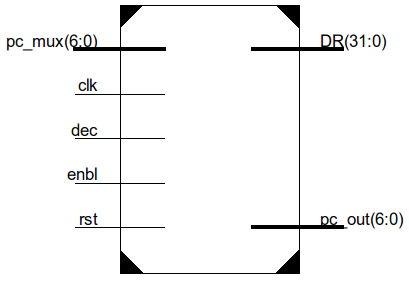
\includegraphics[scale=0.35]{Capitulo01/fetchstage}
\caption{Etapa de b\'usqueda}
\label{fig:fetch}
\end{figure}

\subsection{Funcionamiento}
El \texttt{pc} comienza de 0 y este valor entra en la memoria de instrucciones y en un m\'odulo sumador. En la memoria para que utilice la instrucci\'on ubicada en la posici\'on del mismo valor de contador de programa, y en la entrada del m\'odulo sumador se aumenta en 1 el valor para poder avanzar en el pr\'oximo ciclo de clock a una nueva instrucci\'on. Las salidas de esta etapa son la instrucci\'on a ejecutar y el valor del contador de programa.  (ver Figura \ref{fig:fetchzoom})

\begin{figure}[H]
\centering
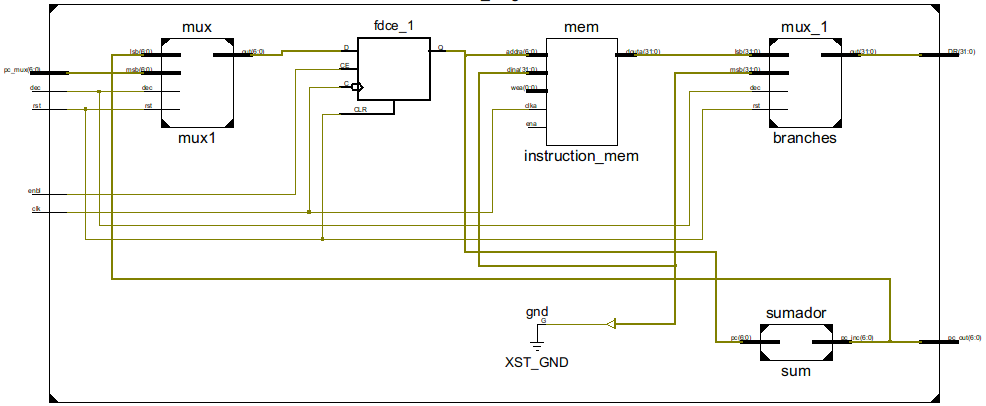
\includegraphics[scale=0.35]{Capitulo01/etapafetchzoom}
\caption{Etapa de b\'usqueda}
\label{fig:fetchzoom}
\end{figure}

\subsection{Multiplexor}

El m\'odulo multiplexor es binario, o sea que solamente elige entre dos valores. En nuestro caso debe escoger entre el \texttt{pc} que viene incrementado desde el m\'odulo sumador o el que viene modificado por un salto desde la etapa de ejecuci\'on. 

\begin{figure}[H]
\centering
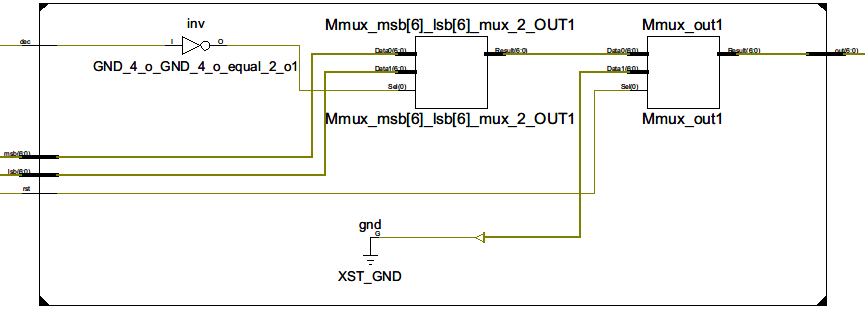
\includegraphics[scale=0.4]{Capitulo01/mux_fig.png}
\caption{M\'odulo multiplexor}
\label{fig:muxmodule}
\end{figure}

En la entrada del multiplexor entran 12 cables para que elija entre la parte alta y la parte baja, dependiendo de si es 1 o 0. Como lo programamos, cuando \texttt{dec} est\'a en uno elige el \texttt{pc}  que viene incrementado. En el otro caso, elige el que esta modificado por la etapa de ejecución.

\begin{figure}[H]
\centering
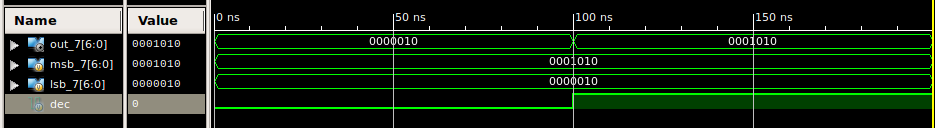
\includegraphics[scale=0.4]{Capitulo01/mux_test}
\caption{Testbench del multiplexor}
\label{fig:muxt}
\end{figure}

\subsection{Incremento}
El m\'odulo sumador simplemente incrementa el \texttt{pc}, tiene solamente una entrada que es un bus de 7 bits y este valor es incrementado dentro del m\'odulo. 


\begin{figure}[H]
\centering
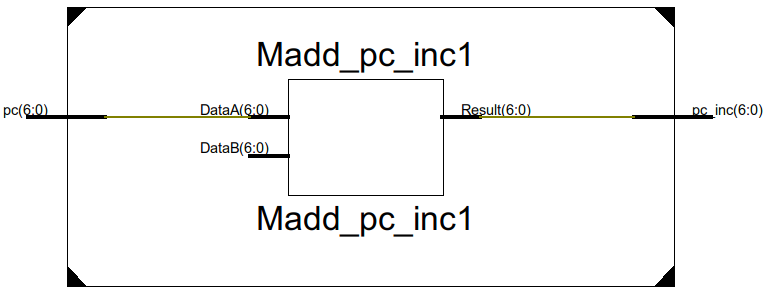
\includegraphics[scale=0.45]{img/sumador_inside}
\caption{Modulo sumador}
\label{fig:sumador}
\end{figure}


En el testbench contador de programa se va modificando de a uno, entonces la salida que en este caso es \texttt{pc\_inc} y esta ingresa en el registro del \texttt{PC}. 


\begin{figure}[H]
\centering
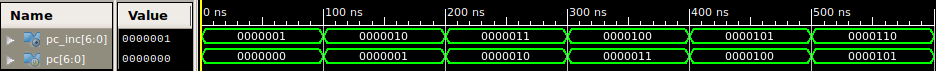
\includegraphics[scale=0.45]{Capitulo01/sum_test}
\caption{Testbench del sumador}
\label{fig:sumt}
\end{figure}


\subsection{Etapa de búsqueda con m\'odulos integrados}
Finalmente generamos un m\'odulo que integra los m\'odulos anteriores y terminamos la etapa. En este clock solamente el registro \texttt{pc} cambiaría de valor. 

\begin{figure}[H]
\centering
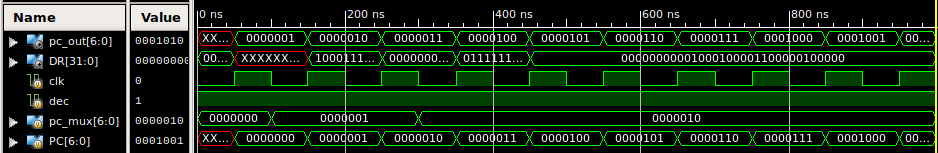
\includegraphics[scale=0.45]{Capitulo01/fetch_test}
\caption{Testbench del modulo fetch}
\label{fig:fetcht}
\end{figure}

Para entender que hace esta etapa podemos ver los cambios en la figura \ref{fig:fetcht}. Debemos comenzar viendo que \texttt{PC} no tiene ning\'un valor y es el que le ingresara en el clock a la memoria de instrucciones, \texttt{pc\_out} tampoco contiene ning\'un valor y este entra en el multiplexor (la memoria de instrucciones se puede ver en \ref{a.coe}).  
En el primer clock ascendente como \texttt{dec} esta en uno, elige \texttt{pc\_mux} para escribir al \texttt{pc} todos ceros, o sea, la primera direccion de memoria. El \texttt{dr}  muestra solo x porque en el clock anterior el \texttt{pc} estaba en x y en la memoria no direcciona en ninguna posici\'on valida. En el pr\'oximo clock ascendente ya el \texttt{pc} contiene ceros por lo que autom\'aticamente \texttt{pc\_out} va a tener el valor de \texttt{PC} + 1, pero \texttt{dec} esta en 1 por lo que sigue eligiendo a \texttt{pc\_mux}, que en el clock descendente anterior ya se le hab\'ia aumentado el valor en 1 por lo que este valor va a ser ingresado en el pr\'oximo clock al \texttt{pc} y \texttt{dr} ya comienza a mostrar el primer valor de la memoria de instrucciones. Los siguientes clocks funcionan de la misma manera.

\lstinputlisting[label=a.coe, caption=Contenido de la memoria de instrucciones, captionpos=b]{Capitulo01/a.coe}	
	\chapter{Latch Etapa de búsqueda - Etapa de decodificaci\'on}
\section{M\'odulo}
Este latch se encarga de mantener el valor de la instrucci\'on y el contador de programa para despues de un clock pasarlo a la siguiente etapa, la etapa de decodificaci\'on.

\begin{figure}[H]
\centering
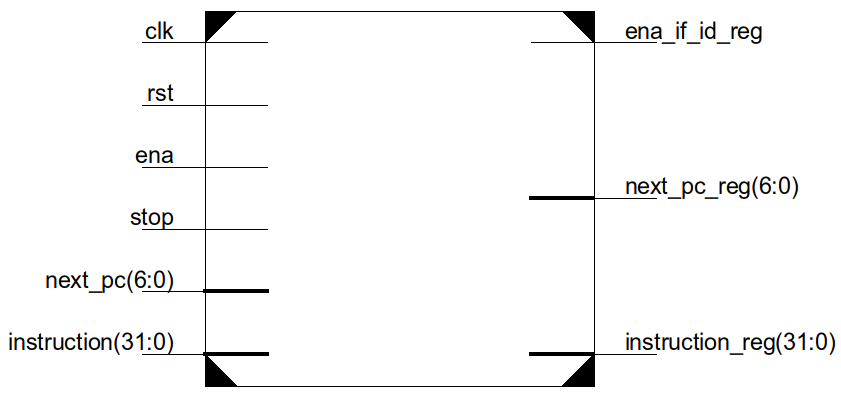
\includegraphics[scale=0.35]{img/latch_if_id}
\caption{Latch etapa de busqueda, etapa de decodificaci\'on}
\label{fig:latchifid}
\end{figure}

Como se puede ver en la figura \ref{fig:latchifid} el latch tiene las siguientes entradas:
\begin{itemize}
  \item \textbf{c
  lk}: Clock que gobierna todo el sistema.
  \item \textbf{rst}: Entrada de reset.
  \item \textbf{ena}: Habilitaci\'on del chip.
  \item \textbf{stop}: A diferencia del ena, esta senal se encarga de retener la instruccion hasta que se d\'e de baja esta senal.
  \item \textbf{next\_pc}: Entrada del contador de programa. El prop\'osito es para utilizarlo en las pr\'oximas etapas por si existe una instrucci\'on de salto para sumarlo a este valor.
  \item \textbf{instruction}: bus de datos que contiene el valor de la instrucci\'on a ejecutar.  
\end{itemize}

Las salidas de este m\'odulo son:
\begin{itemize}
  \item \textbf{ena\_if\_id\_reg}: Pasa a la etapa de decodificaci\'on la senal enable.
  \item \textbf{next\_pc\_reg}: Contador de programa de la etapa de b\'usqueda de la instrucci\'on.
  \item \textbf{instruction\_reg}: Instrucci\'on de la etapa de b\'usqueda.
\end{itemize}

\section{Testbench}
	\section{Etapa de decodificaci\'on}

En esta etapa, mediante la obtenci\'on de la instrucci\'on a trav\'es del latch entre esta etapa y la etapa de b\'usqueda de la instrucci\'on, se procede a activar señales y separar los datos para que se ejecute la instrucci\'on proporcionada de manera correcta.
Las entradas a esta etapa se pueden ver en la figura \ref{fig:decode}.

\begin{figure}[H]
\centering
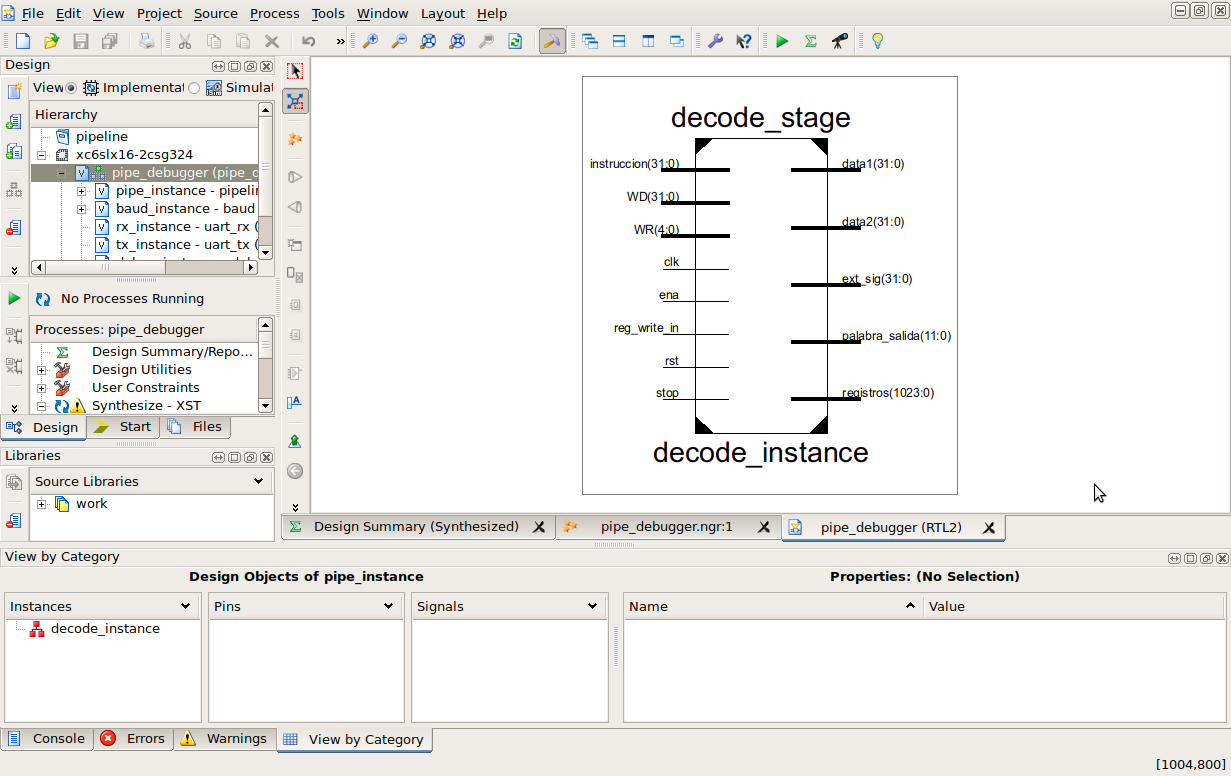
\includegraphics[scale=0.5]{img/decode_stage}
\caption{Etapa de decodificaci\'on}
\label{fig:decode}
\end{figure}

 
Las entradas son: 
\begin{itemize}
  \item \textbf{instrucci\'on}: Bus de 31 bits de ancho que contiene todo lo necesario para que se ejecute la etapa de decodificaci\'on.
  \item \textbf{WD}: Datos que se van a escribir en el banco de registros en WR.
  \item \textbf{WR}: Registro que se va a escribir el dato WD.
  \item \textbf{clk}: Clock general del sistema.
  \item \textbf{ena}: Señal de habilitaci\'on del m\'odulo.
  \item \textbf{reg\_write\_in}: Señal que habilita la escritura de un registro del banco de registros.
  \item \textbf{stop}: Señal que para la ejecuci\'on y el funcionamiento normal del m\'odulo en caso de que exista alg\'un branch o jump. 
\end{itemize}

Esta etapa contiene m\'odulos que son fundamentales para su funcionamiento, la etapa m\'as en detalle se puede ver en la figura \ref{fig:decodedetail}, estos m\'odulos son la unidad de control, el banco de registros, la unidad de extensi\'on de signo y un multiplexor.

\begin{figure}[H] 
\centering
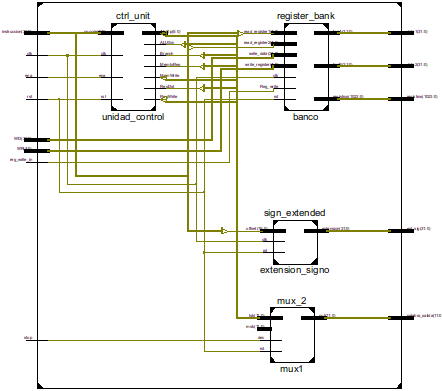
\includegraphics[scale=0.7]{img/decode_stage_inside}
\caption{Detalle etapa de decodificaci\'on}
\label{fig:decodedetail}
\end{figure} 

\subsection{Unidad de control}
La unidad de control se encarga de tomar la parte mas alta de la palabra y decodificar el tipo de instrucci\'on (ver figura \ref{fig:ctrl_unit}) para activar o desactivar señales que se encargan de activar o desactivar multiplexores y otros m\'odulos.

\begin{figure}[H]
\centering
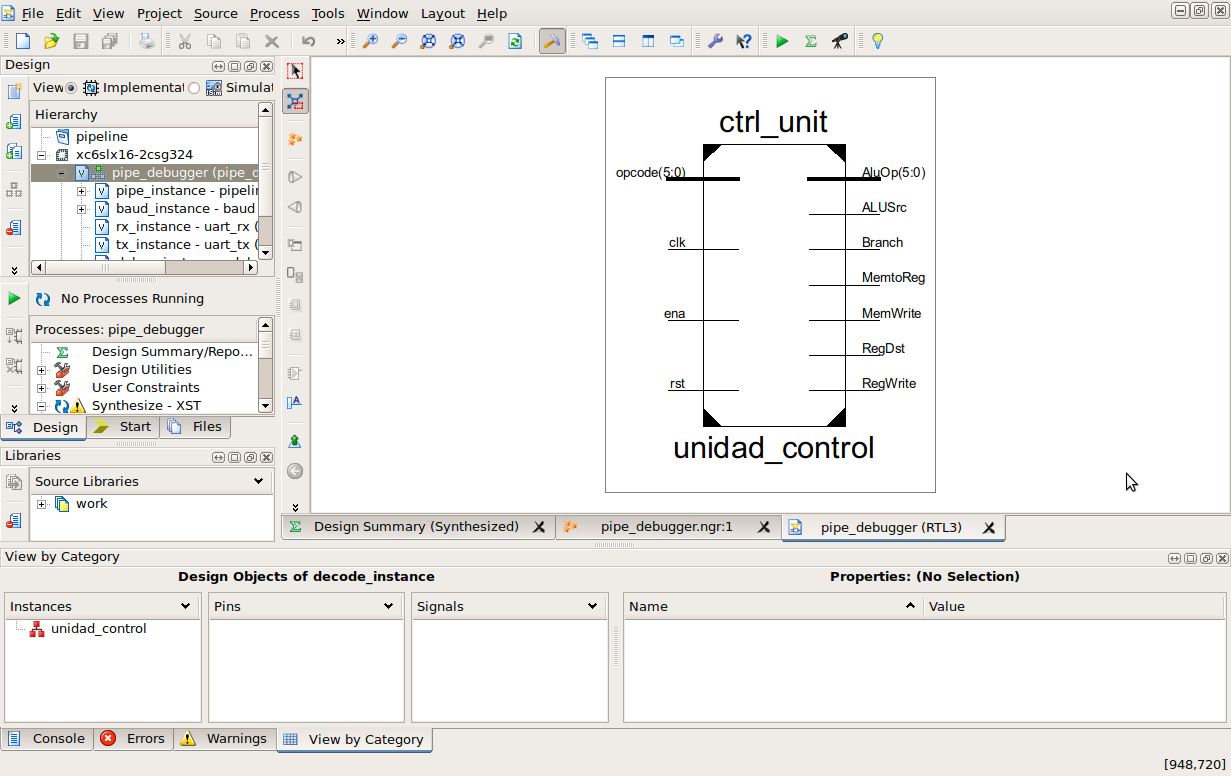
\includegraphics[scale=0.5]{img/unidad_control}
\caption{Unidad de control}
\label{fig:ctrl_unit}
\end{figure} 

Tiene como entradas:
\begin{itemize}
  \item \textbf{opcode}: Bus de 6 bits que es la parte alta de la instrucci\'on.
  \item \textbf{clk}: Clock general del sistema.
  \item \textbf{ena}: Entrada de habilitaci\'on del chip.
  \item \textbf{rst}: Entrada de reset del chip.
\end{itemize}

Y las salidas:
\begin{itemize}
  \item \textbf{aluOp}: Bus de 6 bits que llega a la etapa de ejecuci\'on, pasando antes por el latch hacia la unidad de control de la alu, que sirve para decirle a la alu que operaci\'on l\'ogica realizar.
  \item \textbf{aluSrc}: Cable que va a un multiplexor en la etapa de ejecuci\'on que elige que tipo de dato va a entrar a la alu.
  \item \textbf{Branch}: Señal que se activa en caso de que alg\'un salto sea detectado.
  \item \textbf{MemtoReg}: Señal que se activa en caso de que se deban mover datos de memoria hacia registros.
  \item \textbf{MemWrite}: Señal que se activa en caso de que se vaya a escribir en la memoria de datos.
  \item \textbf{RegDst}: Señal que se activa y llega a un multiplexor para decidir que registro se va a elegir para escribir.
  \item \textbf{RegWrite}: Señal que entra en el banco de registros y le indica si debe o no escribir alguno de los 32 registros que posee. 	
\end{itemize}

\subsection{Banco de registros}
El banco de registros es el m\'odulo que se encarga de guardar las variables que el usuario usa para los programas, pueden ser escritos directamente o desde memoria. La figura \ref{fig:registros}muestra en detalle este m\'odulo.

\begin{figure}[H]
\centering
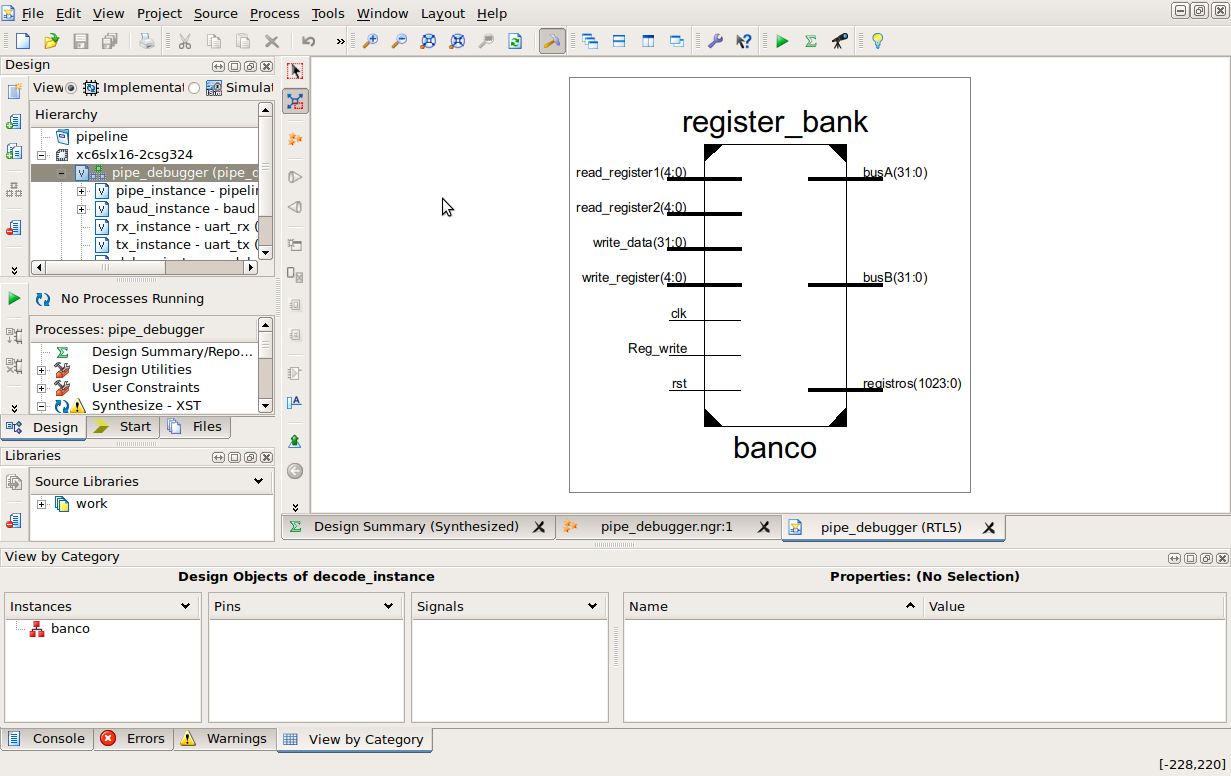
\includegraphics[scale=0.5]{img/banco_registros}
\caption{Banco de registros}
\label{fig:registros}
\end{figure} 

Tiene como entradas:
\begin{itemize}
  \item \textbf{read\_register1}: Bus de 5 bits que indica que registro leer.
  \item \textbf{read\_register2}: Bus de 5 bits que indica que registro leer.
  \item \textbf{write\_data}: Bus de 32 bits que contiene el dato que se va a escribir en el registro si es que est\'a habilitada la senal de escritura de registros (RegWrite).
  \item \textbf{write\_register}: Bus de 5 bits que indica que registro se va a escribir en caso de que est\'e habilitada la señal de RegWrite de la unidad de control.
  \item \textbf{Reg\_write}: Señal que habilita la escritura de un registro del banco de registros.
  \item \textbf{clk}: Clock general del sistema.
  \item \textbf{rst}: Reset del banco que coloca todos los valores de los registros a 0.  
\end{itemize}

Las salidas son:
\begin{itemize}
  \item \textbf{busA}: Bus de 32 bits que da el valor del primer registro elegido en la entrada \textbf{read\_register1}.
  \item \textbf{busB}: Bus de 32 bits que da el valor del primer registro elegido en la entrada \textbf{read\_register2}.
  \item \textbf{registros}: Bus de 1024 bits que sirve para la unidad de debug cuando se deban enviar los valores por la uart.
\end{itemize}

\subsection{Unidad de extensi\'on de signo}
Unidad que se encarga de adaptar al bus de 16 bits de entrada a 32 bits, colocando el signo correspondiente en el \'ultimo bit en caso de que sea un n\'umero negativo el que entre.

\begin{figure}[H]
\centering
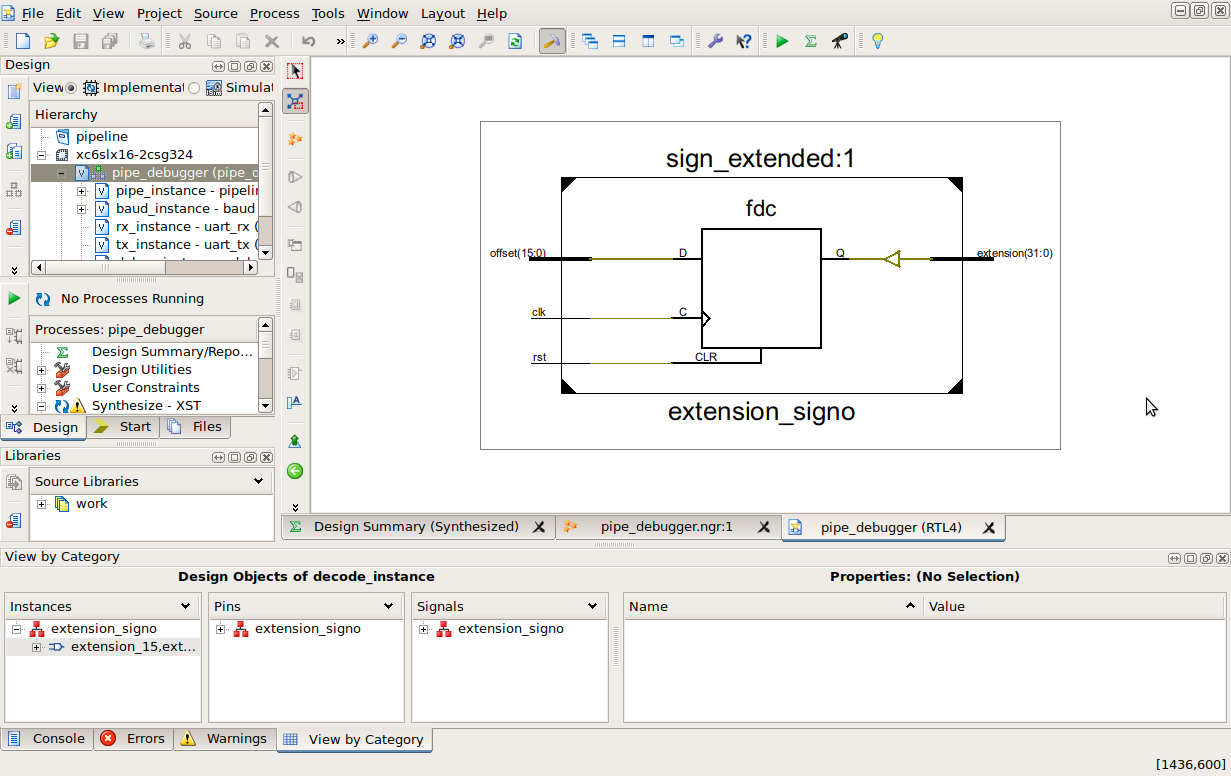
\includegraphics[scale=0.5]{img/extension_signo_inside}
\caption{Unidad de extensi\'on de signo}
\label{fig:sign_extended}
\end{figure}


\subsection{Multiplexor de stop}
Este m\'odulo se encarga, en caso de que la senal de stop est\'e activada, de rellenar con ceros el dato que sale de este modulo que son las senales que activan la unidad de control.

\begin{figure}[H]
\centering
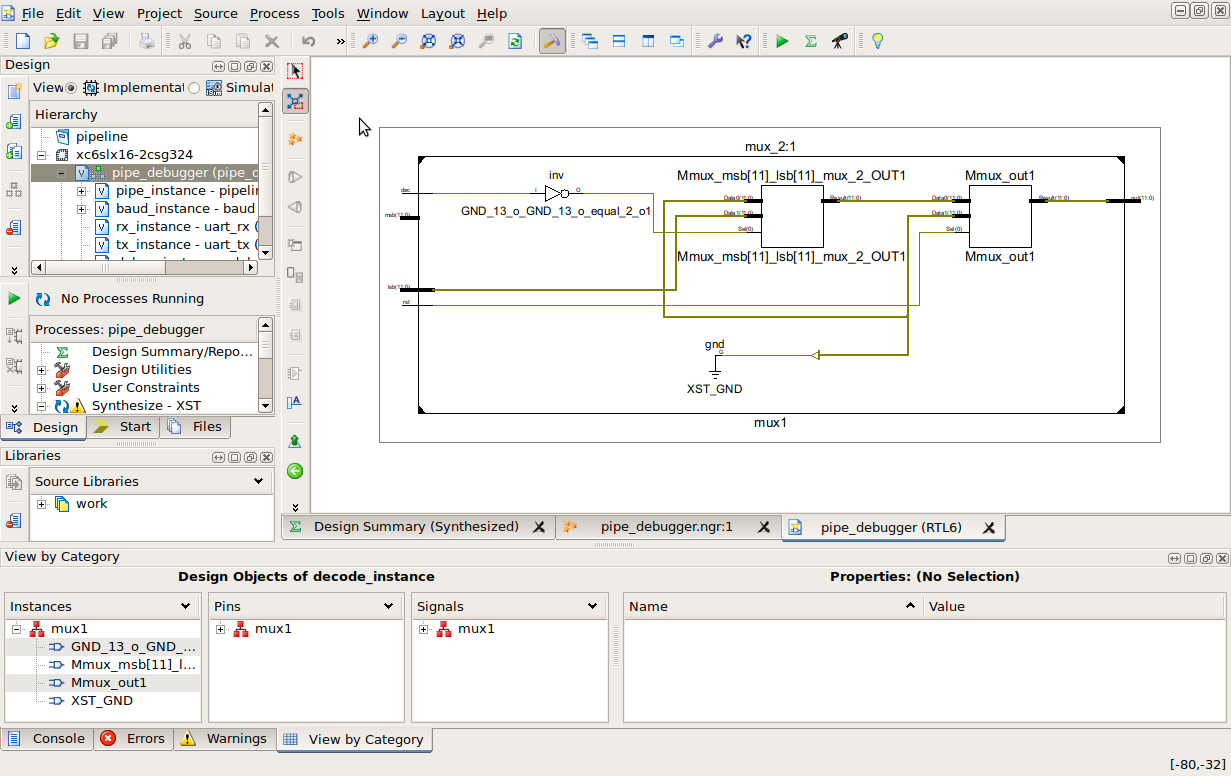
\includegraphics[scale=0.5]{img/multiplexor_inside}
\caption{Multiplexor de señales de la unidad de control}
\label{fig:sign_extended}
\end{figure}

\subsection{Multiplexores de corto}
Las salidas de datos del banco de registros se conectan cada una a un multiplexor. Estos multiplexores trabajan con la unidad de cortocircuito para evitar los riesgos de lectura despues de escritura frente a las etapas de ejecuci\'on, memoria y escritura.

\begin{figure}[H]
\centering
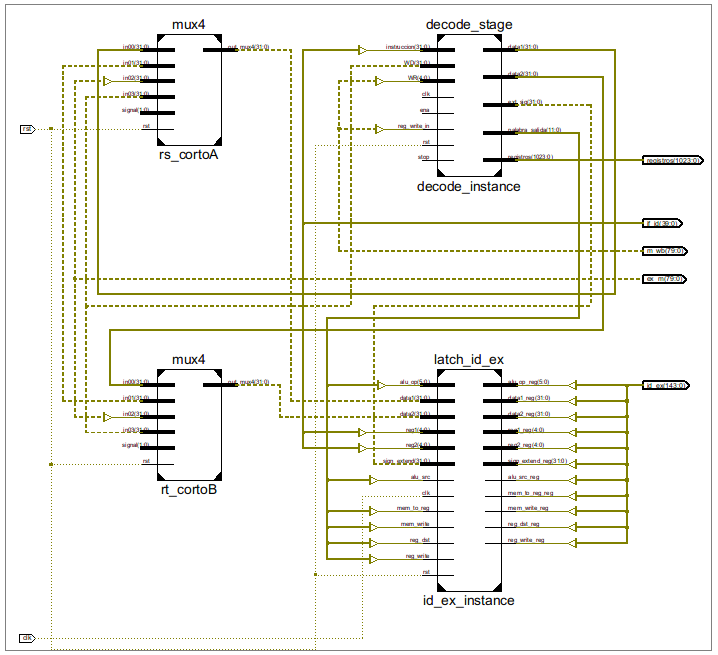
\includegraphics[scale=0.5]{img/cortos}
\caption{Multiplexores de cortocircuito}
\label{fig:corto}
\end{figure}

	\chapter{Latch Etapa de decodificaci\'on - Etapa de ejecuci\'on}
	\section{Etapa de Ejecuci\'on}
Esta etapa se encarga de las operaciones entre los datos que vienen desde el latch, como se ve en la figura siguiente:

\begin{figure}[H]
\centering
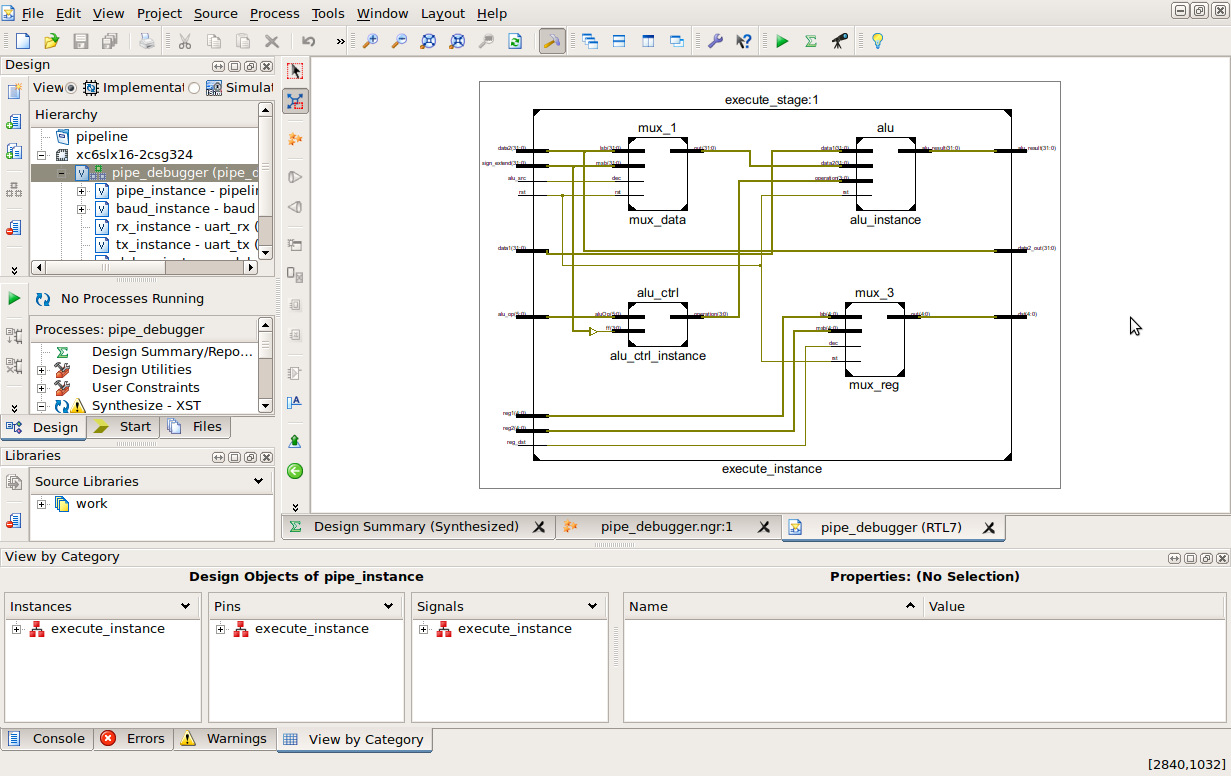
\includegraphics[scale=0.5]{img/execute_stage_inside}
\caption{Etapa de ejecuci\'on}
\label{fig:fetch}
\end{figure}

Esta etapa se encarga de operar con los datos que se le presentan en la entrada, eligiendo la operaci\'on que fue decodificada en la etapa anterior y pasando el resultado a la siguiente etapa.
Tiene como entradas:

\begin{itemize}
  \item \textbf{alu\_op}: Bus de 6 bits que lleva los datos para que la unidad de control de la alu se encargue de elegir que operacion ejecutar.	
  \item \textbf{data1}: Datos que entran a la alu para ser procesados.
  \item \textbf{data2}: Datos que entran en el mux1 para elegir contra sign\_extend y tambien sale directamente hacia el latch.
  \item \textbf{reg1}: Bus de 5 bits que entra a mux\_2 para elegir contra reg2 segun la senal reg\_dst para conocer cual de los registros se va a escribir en el banco de registros en la etapa de escritura.
  \item \textbf{reg2}: Bus de 5 bits que entra a mux\_2 para elegir contra reg1 seg\'un la senal reg\_dst para conocer cual de los registros se va a escribir en el banco de registros en la etapa de escritura. 	
  \item \textbf{sign\_extend}: Extensi\'on de signo que entra en el multiplexor mux\_1 para elegir contra data2 y entrar a la alu para operar.
  \item \textbf{alu\_src}: Señal que elige entre data2 y sign\_extend en el mux\_1
  \item \textbf{reg\_dst}: Señal que elige entre uno de los dos registros en mux\_2 que entran a la etapa para conocer cual se escribe en la etapa de escritura.
  \item \textbf{rst}: Reinicio del m\'odulo. 
\end{itemize}

Tiene los modulos alu y alu\_ctrl.

\subsection{Control de la ALU}
El control de la alu en detalle se muestra en la siguiente figura.

\begin{figure}[H]
\centering
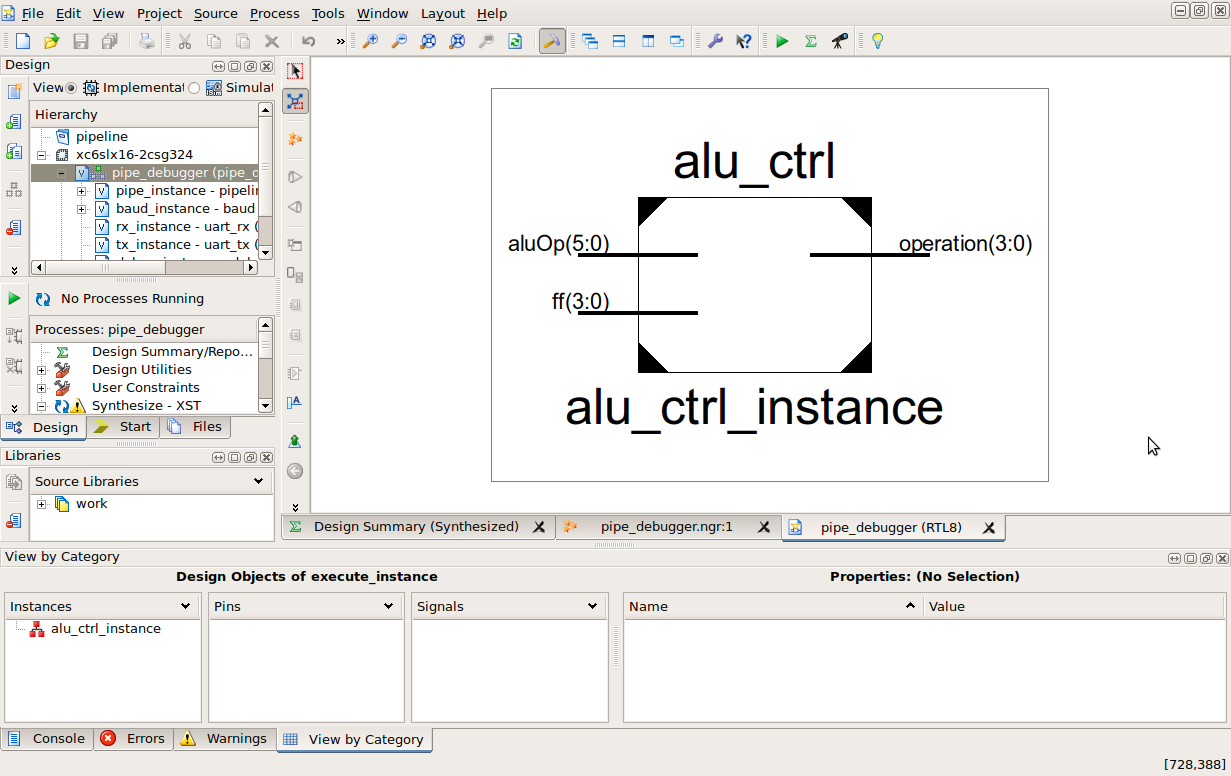
\includegraphics[scale=0.5]{img/alu_ctrl}
\caption{M\'odulo de control de la ALU}
\label{fig:fetch}
\end{figure}

Tiene como entradas:

\begin{itemize}
  \item \textbf{alu\_op}: Opcode que entra a este m\'odulo para decodificar que operaci\'on debe realizar la alu.
  \item \textbf{ff}: Entran 4 bits que provienen de la parte baja extensi\'on de signo y genera el opcode que utiliza la alu para ejecutar la operaci\'on.  
\end{itemize}

Y la salida:
\begin{itemize}
  \item \textbf{operation}: Bus de 4 bits que ingresa a la alu para realizar la operaci\'on correspondiente.
\end{itemize}

\subsection{ALU} 
La ALU es el coraz\'on de esta etapa y es la que se encarga de sumar ejecutar la operacion correspondiente a los operandos suministrados.

\begin{figure}[H]
\centering
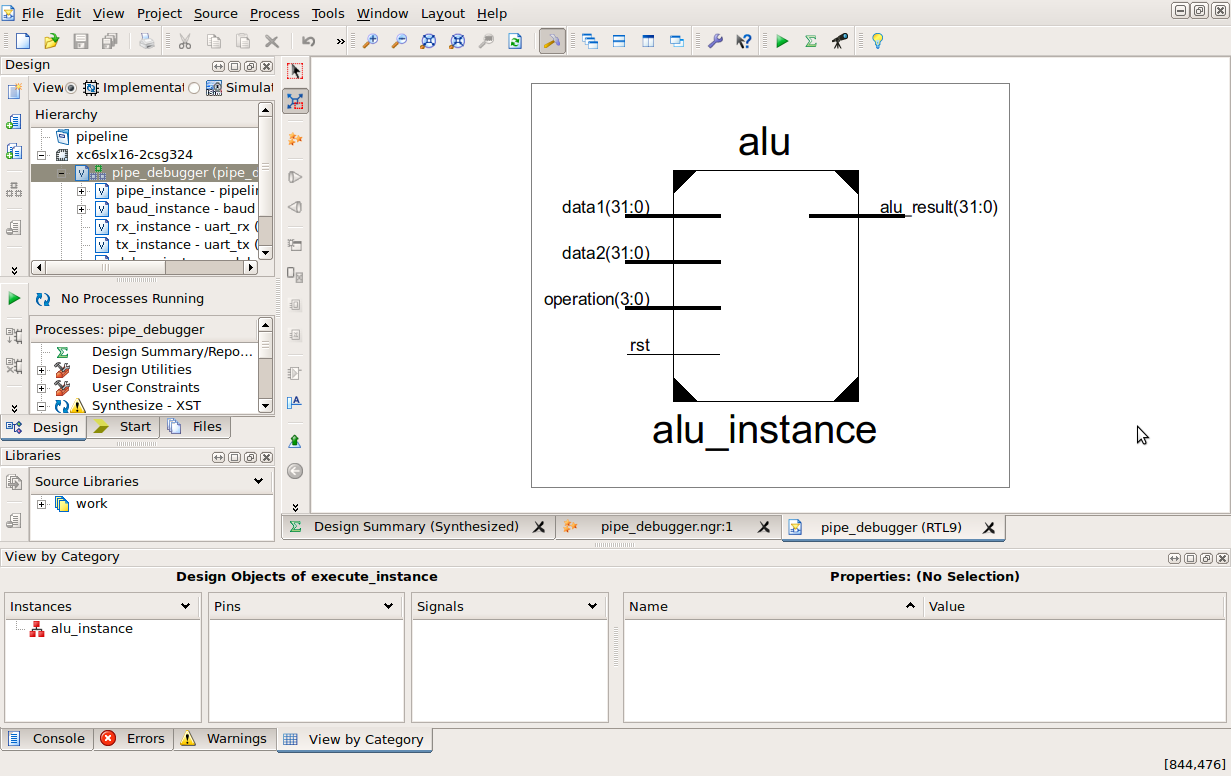
\includegraphics[scale=0.5]{img/alu}
\caption{ALU}
\label{fig:fetch}
\end{figure}

Entradas:

\begin{itemize}
  \item \textbf{data1}: Primer operando.
  \item \textbf{data2}: Segundo operando.
  \item operation: Operaci\'on a realizar con los operandos dentro del m\'odulo.
  \item \textbf{rst}: Señal de reset del m\'odulo.
\end{itemize}

Salida:

\begin{itemize}
  \item \textbf{alu\_result}: Resultado de la operaci\'on realizada entre los operandos.
\end{itemize}

\begin{center}
\begin{table}[H]
%\resizebox*{15cm}{!}{
\scriptsize
\centering
\begin{tabular}[\textwidth]{|l|l|}
\hline
AND & 0000\\
\hline
OR & 0001\\
\hline
SUMA & 0010\\
\hline
XOR & 0100\\
\hline
NOR & 0101\\
\hline
Branch EQUAL & 0110\\
\hline
XOR Inmediato & 1001\\
\hline
SLT & 0111\\
\hline
\end{tabular}
\center
\caption{Tabla de operaciones de la ALU}
\label{tab:test1}
\end{table}
\end{center}

	\section{Latch Etapa de Ejecuci\'on - Etapa de memoria}

Esta latch separa las etapas de ejecuci\'on y memoria.
\begin{figure}[H]
\centering
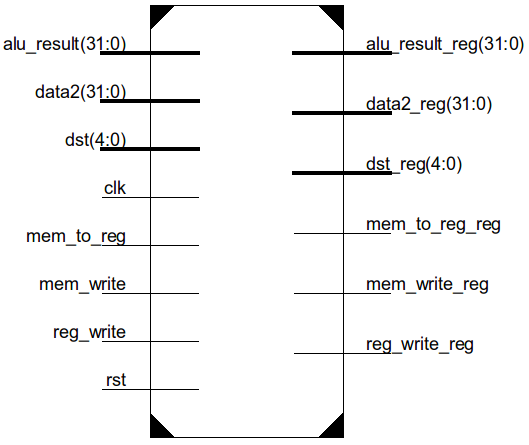
\includegraphics[scale=0.35]{img/latch_ex_m}
\caption{Latche Etapa de ejecuci\'on - Etapa Memoria}
\label{fig:latch_ex_mem}
\end{figure}
Tiene como entradas:
\begin{itemize}
  \item \textbf{alu\_result}: Bus de 32 bits que tiene el resultado de la operaci\'on que se realizo en la ALU.
  \item \textbf{data2}: Bus de 32 bits que es pasado por esta etapa directamente desde el latch anterior, para que las instrucciones que tienen que escribir en la etapa de memoria justamente la memoria de datos la puedan escribir con este valor, siempre y cuando la señal de escritura de memoria este activada.
  \item \textbf{dst}: Registro en el cual se va a escribir en el banco de registros.
  \item \textbf{clk}: Reloj general del sistema.
  \item \textbf{mem\_to\_reg}: Señal que activa la toma de datos de la memoria hacia los registros.
  \item \textbf{mem\_write}: Señal que habilita la escritura en memoria.
  \item \textbf{reg\_write}: Señal que habilita la escritura de los registros.
  \item \textbf{rst}: Señal que pone a cero todos los registros del m\'odulo.
\end{itemize}

Las salidas son las mismas que las entradas anteriores, salvo la señal de reset y la de clock.
	\chapter{Etapa de memoria}
	\section{Latch Etapa de memoria de datos - Etapa de escritura}
Latch que contiene las señales provenientes desde la etapa de decodificaci\'on, y adem\'as el dato que sale de la memoria de datos.

\begin{figure}[H]
\centering
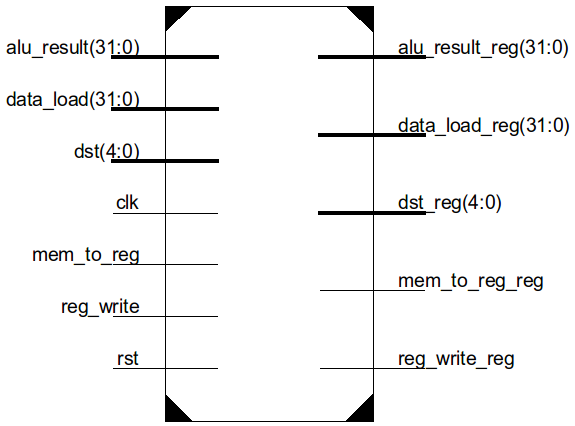
\includegraphics[scale=0.5]{img/latch_m_wb}
\caption{Latch Etapa de memoria - Etapa de Escritura}
\label{fig:latch_m_wb}
\end{figure}

Tiene como entradas:
\begin{itemize}
  \item \textbf{alu\_result}: Bus de 32 bits que toma el resultado que proviene de la operaci\'on de la alu de la etapa de ejecuci\'on.
  \item \textbf{data\_load}: Bus de 32 bits que contiene el dato que fue suministrado por la etapa de lectura de la memoria.
  \item \textbf{dst}: Bus de 5 bits que es el puntero al registro que se va a escribir en el banco de registros de la etapa de decodificaci\'on.
  \item \textbf{clk}: Reloj general del sistema.
  \item \textbf{mem\_to\_reg}: Señal que habilita la escritura del registro a la memoria.
  \item \textbf{reg\_write}: Señal que habilita la escritura de registros de la etapa de decodifici\'on.
  \item \textbf{rst}: Reset que vuelve al estado inicial de los registros. 
\end{itemize} 
	\section {Etapa de escritura}

En esta etapa se ponen en marcha la escritura de registros si es que esa bandera esta habilitada, en otro caso no es una etapa imprescindible, pero necesaria para algunas instrucciones.

\begin{figure}[H]
\centering
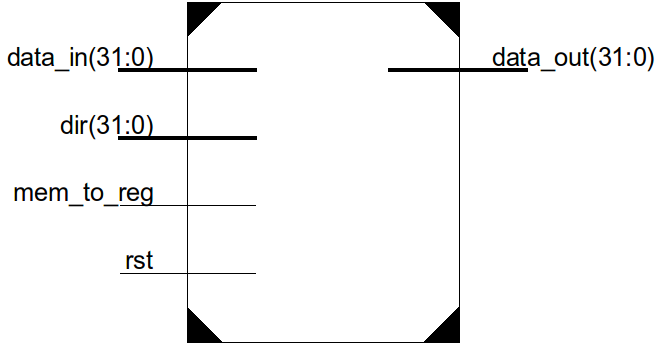
\includegraphics[scale=0.5]{img/wb_stage}
\caption{Etapa de Escritura}
\label{fig:wb_stage}
\end{figure}

Tiene como entradas:
\begin{itemize}
  \item \textbf{data\_in}: Bus de 32 bits que contiene el dato que se obtiene de la memoria.
  \item \textbf{dir}: Datos que se van a escribir en el banco de registros.
  \item \textbf{mem\_to\_reg}: Senal que activa el multiplexor dentro de la etapa y elige entre data\_in y dir.
  \item \textbf{rst}: Reset general del m\'odulo.
\end{itemize}

Salidas:
\begin{itemize}
  \item \textbf{data\_out}: Dato de salida seg\'un la elecci\'on del multiplexor.
\end{itemize}
	\section{M\'odulos adicionales}
Los m\'odulo adicionales son los encargados de dar funcionalidades al pipeline que hacen que mejoren su rendimiento.
\subsection{Unidad de cortocircuito}
M\'odulo que se encarga de detectar si la instrucci\'on siguiente es dependiente de datos de la instrucci\'on anterior. Es decir si el resultado de la instrucci\'on es necesario por las instrucciones siguientes, en ausencia de este m\'odulo hay riesgos de lectura despues de escritura (LDE). En la figura \ref{fig:fwd} se muestra el m\'odulo.

\begin{figure}[H]
\centering
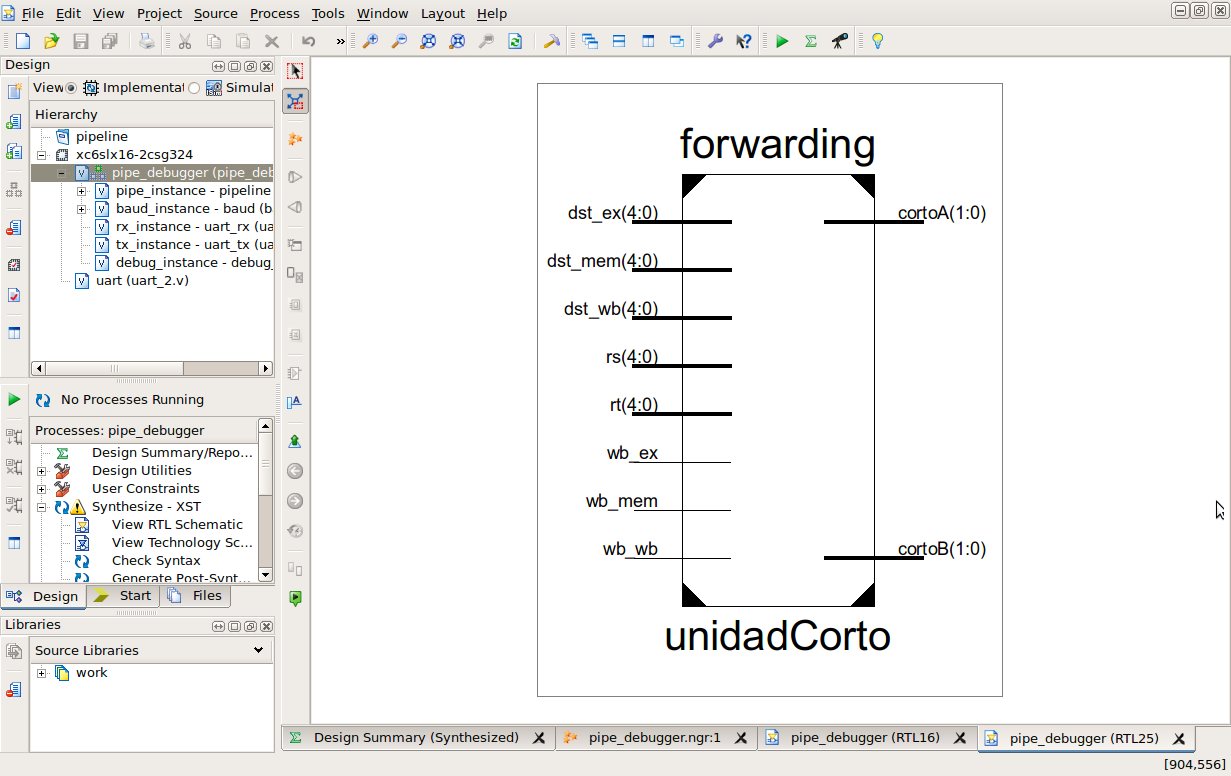
\includegraphics[scale=0.5]{img/forwarding}
\caption{Unidad de cortocircuito}
\label{fig:fwd}
\end{figure}

Tiene como entradas:

\begin{itemize}
  \item \textbf{dst\_ex}: Bus de 5 bits que proviene de la etapa de ejecuci\'on con el valor del registro que se va a escribir.
  \item \textbf{dst\_mem}: Bus de 5 bits que proviene de la etapa de memoria	con el valor del registro que se va a escribir.
  \item \textbf{dst\_wb}: Bus de 5 bits que proviene de la etapa de escritura con el valor del registro que se va a escribir.
  \item \textbf{rs}: Registros de la parte alta que se van a utilizar en la instrucci\'on que actualmente est\'a en la etapa de decodificaci\'on.
  \item \textbf{rt}: Registros de la parte baja que se van a utilizar en la instrucci\'on que actualmente est\'a en la etapa de decodificaci\'on.
  \item \textbf{wb\_ex, wb\_mem, wb\_wb}: Senales de wb que sale del latch para avisar que se va a escribir un registro.  
\end{itemize}

Las salidas del m\'odulo son:
\begin{itemize}
  \item \textbf{cortoA}: Bus de 2 bits que indica si se produjo una dependencia de datos y entra a un multiplexor para que se elija el valor correspondiente cortocircuitado de la etapa en que se detecta el uso de un registro en riesgo para insertarlo en la parte baja de los datos que salen del banco de registros. 
  \item \textbf{cortoB}: Bus de 2 bits que indica si se produjo una dependencia de datos y entra a un multiplexor para que se elija el valor correspondiente cortocircuitado de la etapa en que se detecta el uso de un registro en riesgo para insertarlo en la parte alta de los datos que salen del banco de registros.
\end{itemize}

\subsection{Detector de riesgo}

Este m\'odulo se encarga de actuar en la etapa de decodificaci\'on impidiendo la carga y lectura de una nueva instrucci\'on. Para que se de este caso la instrucci\'on en la etapa de ejecuci\'on debe ser del tipo load, el registro de destino del load coincida con los registro de la siguiente intrucci\'on. Si se dan estas condiciones entonces existe riesgo y es necesario parar el pipeline insertando una burbuja. El m\'odulo se muestra en la figura \ref{fig:datahazard}.

\begin{figure}[H]
\centering
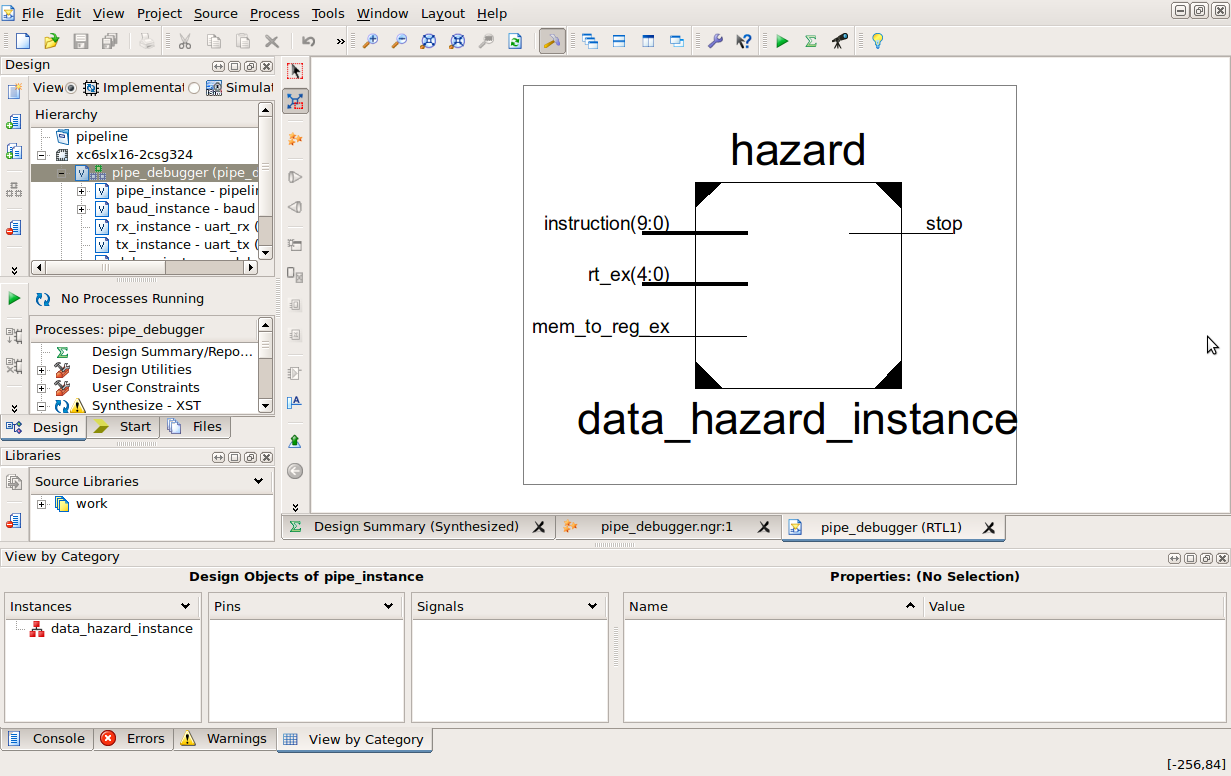
\includegraphics[scale=0.35]{img/data_hazard}
\caption{Detector de riesgo}
\label{fig:datahazard}
\end{figure}  

Las entradas a este m\'odulo son:
\begin{itemize}
  \item \textbf{instruction}: Bus de 10 bits en donde se encuentran los dos registros que pueden sufrir un riesgo a causa de un load.
  \item \textbf{rt\_ex}: Registro que la instrucci\'on del load va cargar.
  \item \textbf{mem\_to\_reg\_ex}: Senal que alerta que se va a cargar un registro desde memoria. 
\end{itemize}

La salida es una senal de \textbf{stop} que va a ser utilizada en el contador de programa para que este no avance y en el latch entre la etapa de b\'usqueda y decodifici\'on. 
	\section{UART}
Como se hizo la uart
	\appendix
\chapter{Etapa de búsqueda}
\lstinputlisting[label=mux, caption=Modulo multiplexor, captionpos=b]{apendice/fetch/mux_7bit.v}
\lstinputlisting[label=mux_test, caption=Test del modulo multiplexor, captionpos=b]{apendice/fetch/mux_test.v}
\lstinputlisting[label=sum, caption=Modulo sumador, captionpos=b]{apendice/fetch/sumador.v}
\lstinputlisting[label=sum_test, caption=Test del modulo sumador, captionpos=b]{apendice/fetch/sumador_test.v}
\lstinputlisting[label=fetch, caption=Modulo fetch, captionpos=b]{apendice/fetch/fetch_stage.v}
\lstinputlisting[label=fetch_test, caption=Test del modulo fetch, captionpos=b]{apendice/fetch/fetch_test.v}
%--------------------------------------------------------
% Apendice
%--------------------------------------------------------
	%\input{}

%--------------------------------------------------------
% Bibliografia
%--------------------------------------------------------
	\begin{thebibliography}{9}
 		 \bibitem{bib:Coad} Computer Organization and design - David A. Paterson, John L. Hennessy
 		 %\cite{ref} para referenciar en el texto
	\end{thebibliography}
	
	\section*{Lista de Acrónimos}\medskip
	\begin{acronym}[SIGCOMM]
		\acro{pc}[PC] {contador de programa}
		\acro{dr}[DR] {registro de datos}
	\end{acronym}
	
%--------------------------------------------------------
% Fin del documento
%--------------------------------------------------------

\end{document}